\subsection{Concurrent Hash-Table}
Our concurrent hash-table is not deviated very much from conventional
concurrent hash-table. We however find opportunity to optimize further by taking 
advantage of some semantics requirement that we have mentioned.

Firstly, we use a spinlock per bucket. This is an viable option since we could
control the table size to reduce the hash collision to minimal. The table size is
related directly to how many concurrent operations which is controlled by 
our packet pool size. When there is no collision, the conflict can only happen
between communication server and a thread when both try to insert into the same
bucket at the same time. With a small number of conflicts, a spinlock is
sufficient for synchronization and allow a very simple design.

Secondly, we design each bucket as an 4-entry array. Each entry consists of two
64-bit words. Within each 4-entry, one entry will be used as \textit{control
entry} and the other three are used for \textit{data entry}. The control entry
has an atomic flag for spin locking, and a pointer to point to the next 4-entry
bucket in case we have more than 3 collisions. A data entry consists of two
64-bit words of key and value pair. In total, 4-entry takes 64-bytes and
typically fits in a cache line. Thus we suffer only 1 cache miss when trying to
lock the bucket and the data can be read without more cache misses.

Lastly, the \texttt{insert} operation also returns the address of the
associated entry having the key in memory. This allows the \texttt{empty}
operation to be a single instruction/single memory write to set the value
associated with key to $\bot$. This is only possible when only one thread can
write to an entry key which is true when no concurrent communication with the
same tag is allowed.

In conclusion, with the above optimization, the \texttt{empty} operation is
lock-free and wait-free, costs only 1 memory write. The \texttt{insert}
operation is cache-friendly and is typically wait-free, costs also 1 memory
write in the common case of no hash collision. Including the spin-lock,
our cost can be as low as two memory writes.

\subsection{Thread scheduler}
The thread scheduler in the system need to support at least  the two most
important operations for synchronization purpose: \texttt{ThreadWait} and
\texttt{ThreadSignal}. We provide 3 different implementation of thread
scheduler: POSIX Thread, Argobots, and a customized thread scheduler using
bitvector.

For both POSIX Thread and Argobots scheduler, the two operations are
implemented using \texttt{condition variable}. Condition variable is a generic
container which is used as a building block for many other synchronization
primitives. It typically requires a mutex and a queue traversal to find the
waiting thread. An alternative is to use a busy-waiting synchronization flag
which has lower latency, however this is considered worst for scaling since the
processor spends useless time polling, thus we do not follow this path.

The different between POSIX Thread and Argobots is that the Argobots scheduler
implements User-Level Thread (ULT), which maintains a fixed number of worker
and schedule \textit{light-weight thread} on top of that. The purpose is to
reduce the overhead of context switching because a context-switch in ULT bypass
the kernel and thus lower the latency to less than a hundred cycles.

Additionally, to further show that improving \texttt{ThreadWait} and
\texttt{ThreadSignal} is critical to the algorithm, we design and implement a
specialized thread scheduler based on bit-vector, namely \textit{Fult}. The
context-switching mechanism is similar to that of Argobots. However, rather
than using a queue as traditional ULT - we indicates a schedulable thread by a
single bit. When a worker is created, it is given a unique worker id, denotes
as $\omega$.  When a thread is created by a worker, it is also assigned an
unique id $\Gamma$.  A pair $(\omega, \Gamma)$ uniquely defines a thread in the
system at a point in time. During creation time, the associated $\Gamma$ bit in
its bitvector structure is marked so that when the worker is free it will
attempt to schedule that thread to run. Algorithms \ref{algo:thread} further
describes our scheduling algorithms. 

\begin{algorithm}
  \caption{Thread scheduler}
  \label{algo:thread}
  \begin{algorithmic}[1]
    \Procedure{Scheduling}{$\omega$, V} \Comment{worker, bit-vector}
    \While {!$\omega$.stop} \Comment{loop until user ask to stop}
      \For{word in V}
      \If{word $\ne$ 0}
        \State localWord = 0
        \State AtomicExchg(word, localWord)
        \While {localWord64 $> 0$}
          \State b = FindFirstSet(localWord)
          \State localWord = FlipBit(localWord, b)
          \State ContextSwitch($b$)
        \EndWhile
      \EndIf
      \EndFor
    \EndWhile
    \EndProcedure
  \end{algorithmic}
\end{algorithm}

\begin{algorithm}
  \caption{Thread Operations}
  \label{algo:thread-ops}
  \begin{algorithmic}[1]
    \Procedure{ThreadWait}{}
      \State ContextSwitch($\omega$)
    \EndProcedure
    \\ 
    \Procedure{ThreadSignal}{sync}
      \State AtomicBitSet(sync.$\omega$.V, sync.$\Gamma$)
    \EndProcedure
  \end{algorithmic}
\end{algorithm}

The scheduler works at 64-threads granularity instead of 1-thread
traditionally.  By using an atomic exchange instruction to swap the interested
word to local variable, we are able to continously perform read/write from/to
this variable without accessing the main memory. This is a work-around since we
could not found suitable atomic read-modify-write instructions operating at the bit
level. An improvement in instruction usage could further improve this algorithm.

Algorithms \ref{algo:thread-ops} describes the two thread operations.
\texttt{ThreadWait} simply switch back to the worker scheduler based on current
worker id (i.e. $\omega$) On the other hand, \texttt{ThreadSignal} shall access
the bit-vector and atomically set the bit in the appropriate word based on the
the same information stored in the synchronization object. $\omega$ and
$\Gamma$ are stored in thread local-storage of the worker, and is updated
whenever a new context is switch to.

Note that the algorithm works because it is guaranteed that the scheduler will
see the \texttt{ThreadSignal} after performing \texttt{ThreadWait}.  It is
errornous to perform \texttt{ThreadSignal} multiple times on the same object
since they will be treated as one or more signal depending on the time the
worker looks at the bit-vector. Thus, to support efficient non-blocking
communication and different flavor of \texttt{MPI_Wait*}, we have to build a
more powerful synchronization.  

Iterating over the bit-vector word by word is more expensive when
there is more threads. We eliminate this problem by implement a hierachical design of
bit-vector.  That is, we could use an additional bit-vector as a hint to index
into the original bit-vector. Specifically, each bit in the secondary
bit-vector indicates which word in the first level may have a schedulable
thread. More specifically, \texttt{ThreadSignal} will perform a bit set first
into the first level then a bit set into the second level. The scheduler will
first look into the second level to find a potential word and go directly to
that word to look for schedulable threads. %Recall that the secondary bit-vector
%is shared among a group of threads, thus It can happen that the secondary might
%indicate the thread is schedulable, but when it arrives at the first level the
%thread is already scheduled. However, this situation does not affect the
%correctness since the thread will not be scheduled twice in any situation.
Using this scheme, suppose we allows $s_2$ words in the second level and each
bit represents $s_1$ words in the first level, the total number of threads we
can support is $s_1 \times s_2 \times 64^2$. Typically we can choose $s_1 = s_2
= 8$ since 8 words fit into a cache line. In that case, it allows $256K$
concurrent threads per worker. 

Although fairness could be an issue, our scheduler maintain progress property.
If a thread is marked as schedulable, it's eventually will be scheduled in a
bounded number of steps. To show that this is true, consider the atomic
exchange as taking a snapshot of the global state. In this snapshot, if a
thread is marked it will be scheduled after all threads having smaller index
are scheduled, which is bounded by the maxmimum number of allowed concurrent
threads decided by the size of the bit-vectors.

\subsection{Concurrent Packet Pool}
In general, the packet pool can be implemented using a lockfree stack. A pool
\texttt{ret} is translated to a stack \texttt{push}, and \texttt{get} is
translated to a stack \texttt{pop}. At the initialization, a fixed number of
packet is initialized from the main memory and \texttt{push} to the container.
The Last-In-First-Out (LIFO) property allows good temporal locality for
writing/reading to/from the content of a data packet. In a single-threaded
environment this design is sufficient for good performance, but not for the
case of multi-core/multi-threaded. Consider a packet recently being used by a thread
and returned to the pool, this packet could be subsequently obtained by a different thread
running in a different core. This leads to several cache misses since the cacheline
is momently owned by the first thread. An example is when two threads running in 
two different cores alternatively perform \texttt{MPI_Send}.

\begin{figure}[t]
  \centering 
  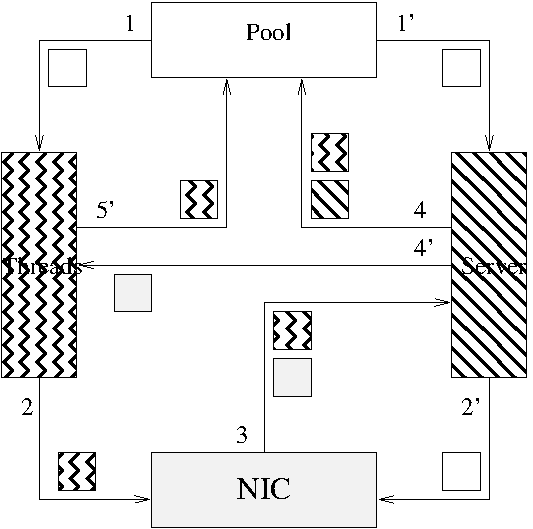
\includegraphics[width=0.3\textwidth]{fig/packetlife.pdf}
  \caption{Packet life cycle: (1) A thread sending data obtain a packet from the
    pool; (2) The thread writes data into the packet and submit it to the NIC;
    (1', 2') Communication server obtains a packet for receiving data
    and posts the packet to the NIC;
    (3) The server polls the NIC and obtains the packet back (either send/recv packet).
    (4) If the packet is for sending, it is returned to the pool;
    If the packet is for receiving and there is a request, the server copies the data
    and returns the packet to the pool;
    (4') If the packet is for receiving and the there is no request, the packet is inserted to hash-table.
    (5') The thread takes packet from the hash-table copies the data before returning it back to the pool.}
  
  \label{fig:packetlife}
\end{figure}

Figure \ref{fig:packetlife} explains how different components in our system
might change the affinity of data inside a packet. The figure shows the life of
a packet from the time it leaves the pool until it is returned. As explained in
the figure, when a packet returns to the pool, it can only has the affinity
of either the communication server or one of the worker thread. More specifically,
if the packet is used for sending data, it shall have the locality of the thread;
if the packet is used for receiving data, it shall have the locality of either
the thread or the server depending on whether the associated request and the
packet is received first. Moreover, when the packet is posted by the server
to the NIC for receiving data, the packet shall lose any affinity it has since
the NIC will perform a write over the packet.

Analysing the packet life cycle naturally motivates us a new design for the
packet pool: split the centralized packet management into a private pool per
worker. Initially, there is a fixed number of packets for each of the pool. At
runtime, we allow moving packets among those pools via \textit{resource-stealing}.

The private pool consists of packets that are identified as having affinity of
the associated hardware thread. It is implemented as a fixed size double-ended
queue (deque). The deque has three main operations: \texttt{popTop},
\texttt{pushTop}, and \texttt{popBottom} which allows LIFO accessing at the one
end and taking items from the other end. The idea is that at the bottom of the
deque are packets that are least recently used and are better candidates for
other purposes. 

When a packet is needed, a \texttt{popTop} is performed with the private pool
of the current worker, which guarantees giving the last packet that was read or
written by the same worker. If the private pool is empty, It performs a
\textit{steal} by randomly chosing another private pool and perform the
\texttt{popBottom} operation. Our algorithms essentially performs
resource-balancing among the set of packets by moving it around pools with the
locality taken into account. Currently we implement the pool using a simple
fixed-size ring-buffer with a spinlock.
